
\chapter{Разработка программы решения теоретико-графовой задачи на
  языке программирования, предназначенном для обработки семантических
  сетей}

\section{Задание}

На этом этапе выполнения расчетной работы вам необходимо будет
разработать программу на языке программирования, предназначенном для
обработки семантических сетей, которая бы решала вашу
теоретико-графовую задачу на основе формализации предметной области,
проведенной на 1-ом этапе. На втором этапе вы должны были написать
программу на С++ с использованием программной модели sc-памяти. Если
на втором этапе вы написали программу с обработкой информации только в
sc-памяти, то данный этап для вас будет очень простым.

В качестве тестов для написанной программы необходимо использовать
тестовые примеры, которые вы сделали в ходе 1-го этапа расчетной
работы.

\section{Установка и настройка рабочей среды}

Сперва мы установим и настроим рабочую среду для программирования на
языке SCP (Semantic Code Programming) и запустим программу-пример
поиска одного из минимальных путей. Всё описанное в этой главе
программное обеспечение находится на кафедральном сервере info в папке
\verb|\\Info\StudInfo\~Методическое обеспечение кафедры\~Учебные курсы\2 курс\ППвИС\@Расчётная работа|. Поэтому в дальнейшем я не буду
указывать полный путь для программного обеспечения и исходных текстов,
а буду ссылаться на эту папку. Нам пригодится модуль sc-core, который
мы устанавливали на 2-ом этапе расчетной работы. Напомню, что я ставил
его в папку \verb|c:\sc-core| и именно этот путь буду использовать в
дальнейшем. Но базу знаний с программой-примером необходимо обновить,
поэтому удаляем папку \verb|c:\sc-core\examples\fs_repo_src| и
копируем папку \verb|fs_repo_src| с сервера \verb|info| в
\verb|c:\sc-core\examples|.

Среда разработки для языка SCP написана как плагин к платформе
Eclipse, поэтому сначала нам необходимо поставить Java Development
Kit. Берем с сервера info установщик \verb|jdk-6u29-windows-i586.exe|
и инсталлируем это ПО. Теперь берем архив
\verb|eclipse-scpdev-3.6.2-win32.zip| с сервера info и разархивируем
его, например, в \verb|d:\tools\|. После этого запускаем исполняемый
файл \verb|d:\tools\eclipse\eclipse.exe|.

С самого начала работы со средой Eclipse она попросит вас указать путь
к рабочему пространству (workspace), в котором будет происходить
создание проектов. Я указал путь \verb|d:\workspace|
(см. рис.~\ref{fig:Setup_Select_workspace}). Нажимаем OK.

\begin{figure}[h!]
  \centering
  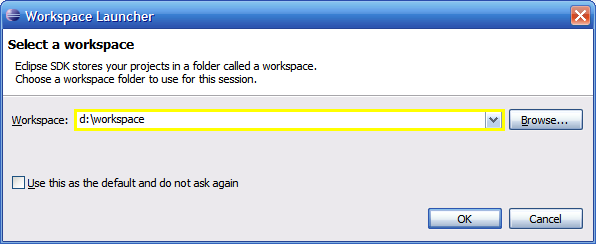
\includegraphics[scale=0.7]{images/5/setup/1_Select_workspace}
  \caption{Выбор рабочего пространства}
  \label{fig:Setup_Select_workspace}
\end{figure}

Среда Eclipse запустилась, и сразу же закройте вкладку
\texttt{Welcome}. Теперь настроим среду выполнения для работы с
проектами баз знаний. Для этого выбираем пункт меню \texttt{Window ->
  Preferences}. Выбираем пункты \texttt{SCP -> SCP Enviroment}. Там
снимаем флажок и указываем путь к корневой директории модуля
\texttt{sc-core} (в моем случае это \verb|c:\sc-core|) как показано на
рис.~\ref{fig:Setup_Setup_scp_enviroment}. Нажимаем кнопки
\texttt{Apply} и затем \texttt{OK}.

\begin{figure}[h!]
  \centering
  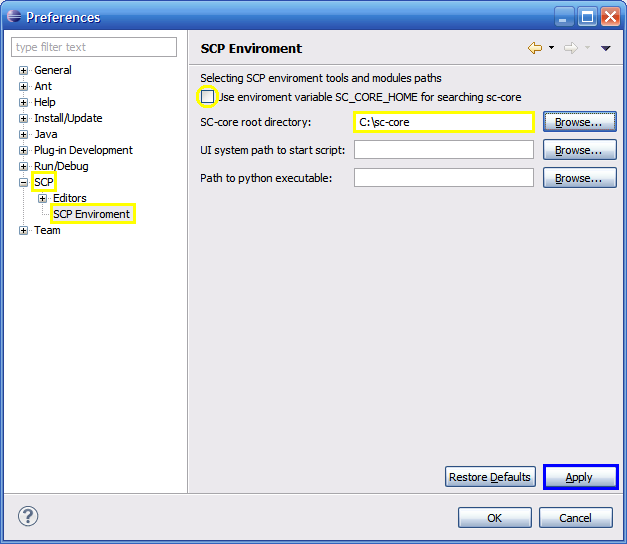
\includegraphics[scale=0.7]{images/5/setup/2_Setup_scp_enviroment}
  \caption{Настройка среды исполнения}
  \label{fig:Setup_Setup_scp_enviroment}
\end{figure}

Пришло время создать проект с примером программы поиска минимального
пути.  Выбираем пункт меню \texttt{File -> New -> Project} и затем
выбираем тип проекта \texttt{SC Repository} в папке \texttt{SCP
  Development}
(см. рис.~\ref{fig:Setup_Select_project_type}). Нажимаем на
\texttt{Next}. На этой странице мастера по созданию проекта
(см. рис.~\ref{fig:Setup_Setup_project}) вводим имя проекта
\verb|wave_find_path| и путь к папке с исходными текстами базы знаний
\verb|c:\sc-core\examples\fs_repo_src| (вспомните, что именно сюда мы
копировали наш пример). Нажимаем кнопку \texttt{Finish}.

\begin{figure}[h!]
  \centering
  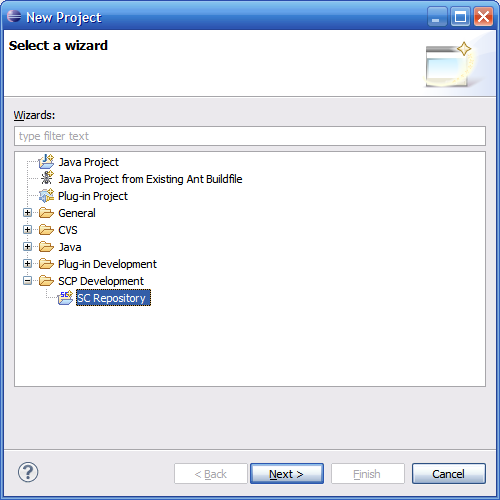
\includegraphics[scale=0.7]{images/5/setup/3_Select_project_type}
  \caption{Выбор типа проекта}
  \label{fig:Setup_Select_project_type}
\end{figure}

\begin{figure}[h!]
  \centering
  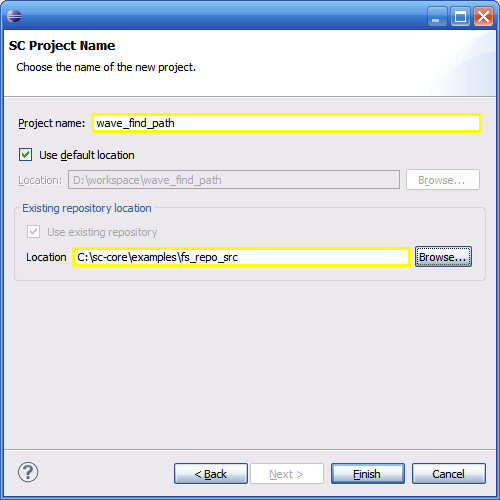
\includegraphics[scale=0.7]{images/5/setup/4_Setup_project}
  \caption{Настройка проекта при создании}
  \label{fig:Setup_Setup_project}
\end{figure}

\begin{figure}[h!]
  \centering
  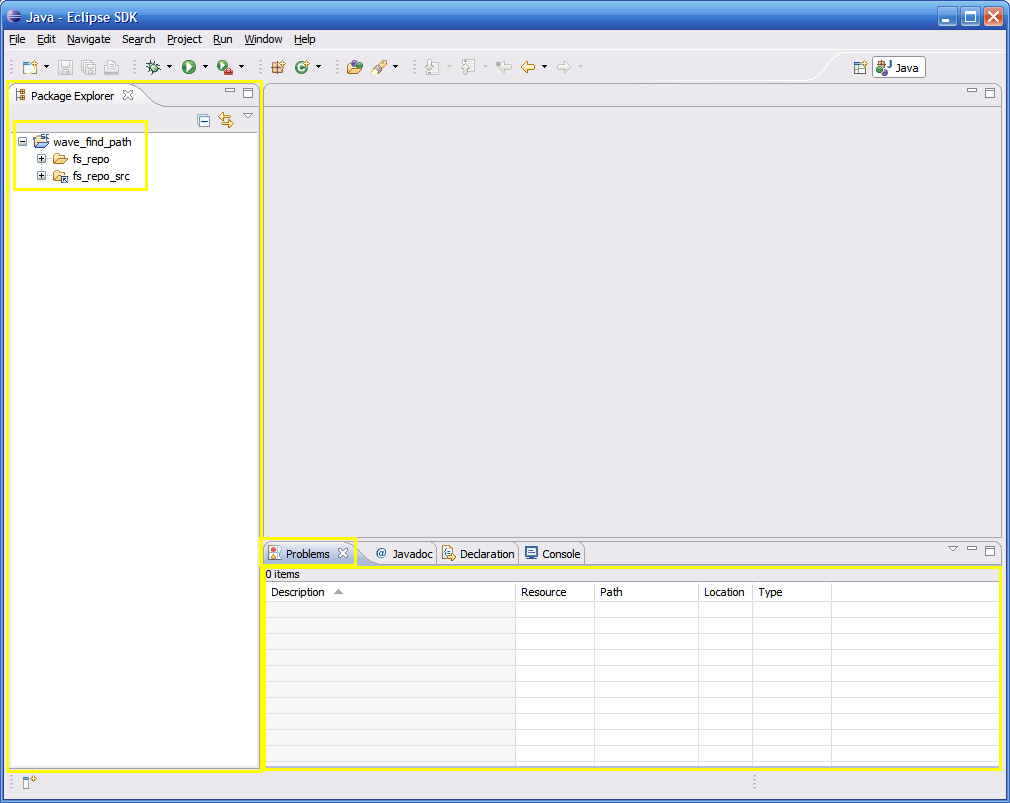
\includegraphics[scale=0.5]{images/5/setup/5_Project_created}
  \caption{Проект wave\_find\_path создан и собран без ошибок}
  \label{fig:Setup_Project_created}
\end{figure}

Проект создан и должен был быть автоматически собран
(см. рис.~\ref{fig:Setup_Project_created}).  Обратите внимание, что на
вкладке Problems таблица пустая. Т.е. сборка произошла без ошибок. Еще
необходимо обратить внимание на две папки в проекте
\verb|wave_find_path|. Они всегда присутствуют в проекте типа
\texttt{SC Repository}. В папке \verb|fs_repo_src| хранятся исходные
тексты базы знаний (в том числе и программы), а папку \verb|fs_repo|
является скомпилированной версией \verb|fs_repo_src|. Содержимое этих
двух папок мы рассмотрим в следующем разделе, а сейчас запустим
программу-пример.

Для запуска проекта в \texttt{Eclipse} необходимо создать конфигурацию
запуска. Вызовем диалог создания конфигурации запуска так, как
показано на рис.~\ref{fig:Setup_Main_run_conf_dialog}, или выбрав
пункт меню \texttt{Run -> Run Configurations$\dots$}

\begin{figure}[h!]
  \centering
  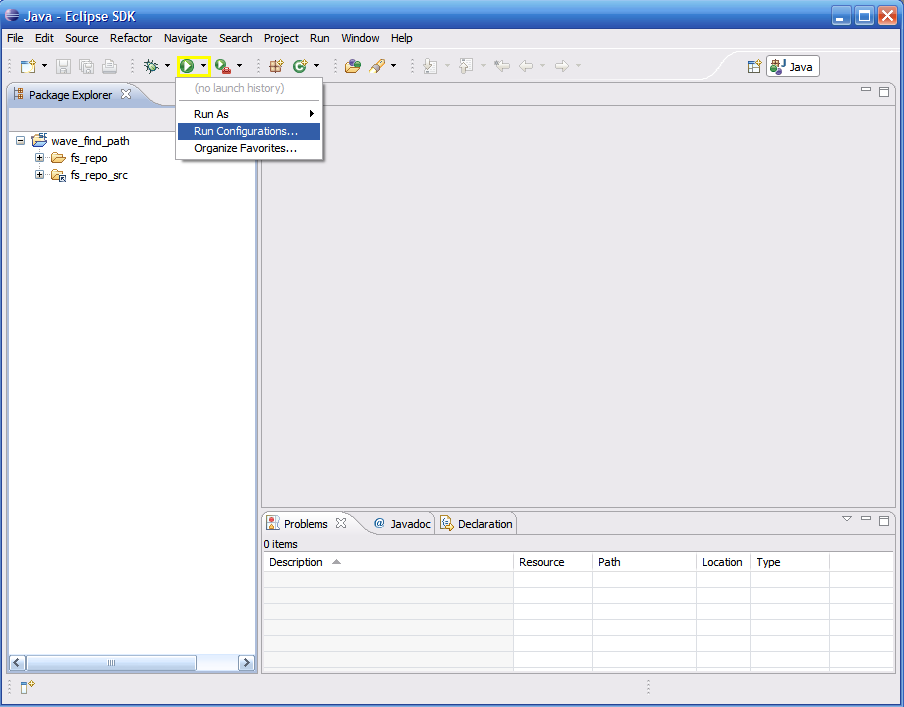
\includegraphics[scale=0.5]{images/5/setup/6_Main_run_conf_dialog}
  \caption{Вызов диалога создания конфигурации запуска}
  \label{fig:Setup_Main_run_conf_dialog}
\end{figure}

Тип конфигурации для запуска scp-программ из консоли называется
\texttt{<<Run with start-pm>>}. Нажимаем правой клавишей мыши на этом
пункте и выбираем \texttt{New}
(см. рис.~\ref{fig:Setup_Select_run_with_start_pm}). Теперь необходимо
настроить созданную конфигурацию.

\begin{figure}[h!]
  \centering
  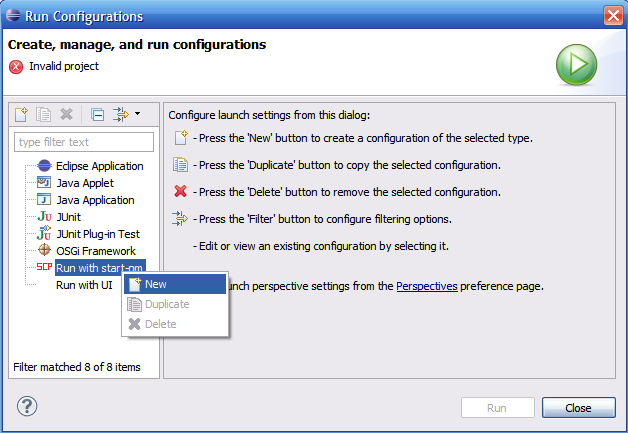
\includegraphics[scale=0.7]{images/5/setup/7_Select_run_with_start_pm}
  \caption{Создание конфигурации запуска из консоли}
  \label{fig:Setup_Select_run_with_start_pm}
\end{figure}

\begin{figure}[h!]
  \centering
  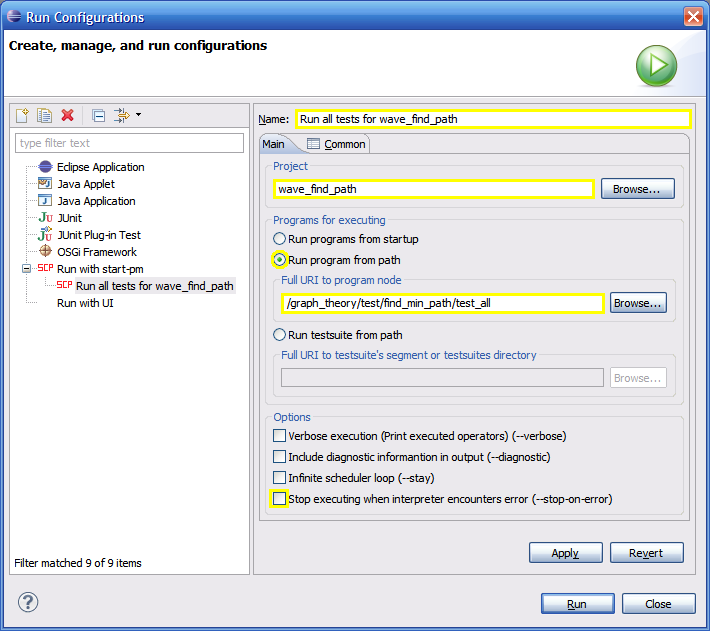
\includegraphics[scale=0.7]{images/5/setup/8_Setup_run_with_start_pm}
  \caption{Настройка созданной конфигурации запуска}
  \label{fig:Setup_Setup_run_with_start_pm}
\end{figure}

На рис.~\ref{fig:Setup_Setup_run_with_start_pm} показана настройка
конфигурации запуска. В поле \texttt{<<Name>>} введено имя
конфигурации \texttt{<<Run all tests for wave\_find\_path>>} (имя
может быть произвольным). В поле \texttt{<<Project>>} необходимо
записать или выбрать из списка при помощи кнопки
\texttt{<<Browse$\dots$>>} имя проекта, для которого будет работать
эта конфигурация. В нашем случае это \verb|wave_find_path|. В блоке
\texttt{<<Programs for executing>>} выбираем \texttt{<<Run program
  from path>>}, т.е. будем запускать программу по URI (данный способ
запуска мы будем использовать всегда). В поле \texttt{<<Full URI to
  program node>>} записываем URI
\verb|/graph_theory/test/find_min_path/test_all| (как получается такой
URI, мы рассмотрим в следующих разделах). Обязательно снимаем галочку
с пункта \texttt{<<Stop executing when interpreter encounters error
  (--stop-on-error)>>} в блоке \texttt{<<Options>>}. Нажимаем
\texttt{Apply} и затем \texttt{Run}. Вы должны увидеть вкладку
\texttt{Console} в нижней части экрана, в которую будет выводиться
информация о выполнении тестовых примеров.

Так как полноценного отладчика scp-программ нет, то для отладки
необходимо использовать конфигурацию запуска, которая показана на
рис.~\ref{fig:Setup_Run_conf_with_verbose_output}. В ней необходимо
установить флажок \texttt{<<Verbose Execution (Print Executed
  Operator) (--verbose)>>}. Нажимаем кнопки \texttt{Apply} и затем
\texttt{Run}. Теперь во вкладке Console должен печататься полный
пооператорный лог выполнения всех вызванных scp-программ.

\begin{figure}[h!]
  \centering
  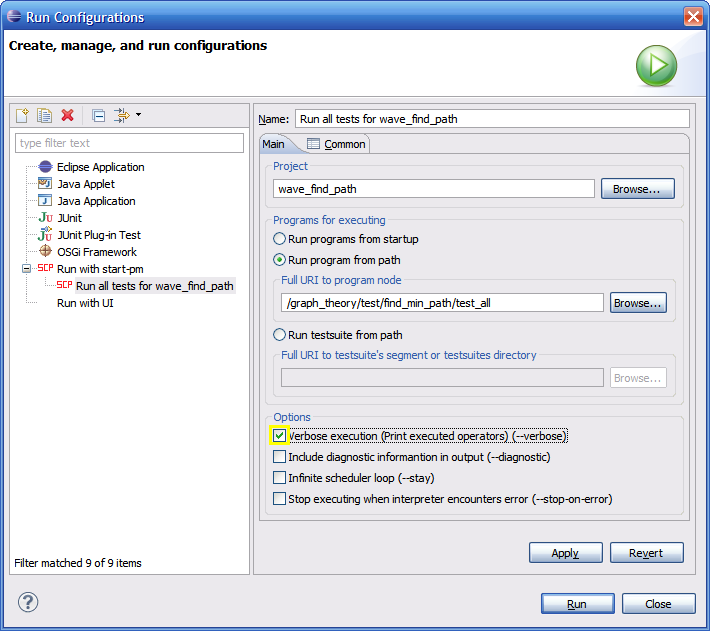
\includegraphics[scale=0.7]{images/5/setup/9_Run_conf_with_verbose_output}
  \caption{Конфигурация запуска из консоли с подробным выводом}
  \label{fig:Setup_Run_conf_with_verbose_output}
\end{figure}

Мы закончили настройку рабочей среды и теперь перейдем к описанию
содержимого исходного и бинарного репозиториев базы знаний.

\pagebreak

\section{Содержимое исходного и бинарного репозиториев базы знаний}

Исходные тексты базы знаний (а к ним относятся и программы на SCP)
хранятся в исходном репозитории, который обычно называется
\verb|fs_repo_src|. Обратите внимание, что в созданном нами проекте
\verb|wave_find_path| такая папка присутствует. Как вы уже знаете, на
данном этапе существования технологии используется реализация
sc-памяти с сегментной моделью. Есть sc-сегменты, в которых
содержаться sc-элементы, и sc-директории, в которых содержатся
sc-сегменты. Для удобства адресации этих трех видов объектов можно
использовать URI (Uniform Resource Identifier). Если кто-то это
подзабыл, то необходимо обратиться к документации по программной
модели sc-памяти из руководства по выполнению 2-го этапа расчетной
работы.

Исходный репозиторий компилируется в папку \verb|fs_repo|. Как вы
заметили, структура sc-памяти с точки зрения сегментной модели имеет
свойство древовидности. Это позволяет хранить содержимое sc-памяти на
файловой системе один в один. URI \verb|/| соответствует корень
бинарного репозитория (папка с именем \verb|fs_repo|). Любой подпапке
в бинарном репозитории \verb|fs_repo| соответствует sc-директория с
тем же именем, а любому файлу в \verb|fs_repo| соответствует
sc-сегмент с тем же именем. Причем URI sc-директорий и sc-сегментов
будет записываться относительно папки \verb|fs_repo|, т.е. корня
репозитория. Таким образом у нас есть исходный репозитория, из
которого получается бинарный репозиторий, на основании которого
формируется содержимое sc-памяти. Рассмотрим подробно исходный
репозиторий.

Каждая папка исходного репозитория будет существовать и в бинарном
репозитории, если в этой папке есть хотя бы один файл, который может
быть оттранслирован в бинарную версию. Исходные файлы бывают трех
типов:

\begin{itemize}
\item Тип файла, при котором для формирования сегмента используются
  имя файла и его положение в исходном репозитории. Например,
  \verb|fs_repo_src/graph_theory/find_min_path.m4scp| будет
  оттранслирован и будет соответствовать
  \verb|fs_repo/graph_theory/find_min_path| в бинарном
  репозитории. Как видите, убирается только расширение. Такие исходные
  тексты могут быть следующего вида (определяется по расширению):
  \begin{itemize}
  \item \texttt{*.scs} – исходные текст на SCs (Semantic Code
    string). Линейная форма представления sc-тектов;
  \item \texttt{*.m4scp} – исходные тексты SCP-программ, транслируемые
    в SCs;
  \end{itemize}

\item Тип файла, для которого не формируется сегмент. Такие исходные
  тексты могут быть следующего вида (определяется по расширению):
  \begin{itemize}
  \item \texttt{*.scsy} – заголовочные файлы синонимом, которые могут
    быть подключены в scs-файлы и m4scp-файлы. В исходном репозитории
    есть особая папка \verb|include|, в которой находятся все
    scsy-файлы. В некотором роде scsy-файл является аналогом
    заголовочного файла в С/С++.
  \end{itemize}

\item Тип файла, который не подлежит обработке. Все файлы, кроме
  перечисленных выше.
\end{itemize}

В следующих разделах мы рассмотрим форматы scs-, scsy- и m4scp-файлы.

\section{Язык SCs для представления sc-конструкций в линейном виде}

В файлах с расширением scs должен содержаться текст на языке SCs. Так
же, как существует графический язык для записи sc-конструкций SCg,
существует и текстовый язык для записи sc-конструкций SCs.

Текст на языке SCs состоит из sc.s-предложений. Каждое
sc.s-предложение должно заканчиваться точкой с запятой <<\texttt{;}>> и
простейшим видом такого предложения является:
\begin{verbatim}
/* Это комментарий */
element; // Это тоже комментарий
\end{verbatim}

Такое scs-предложение будет соответствовать
рисунку~\ref{fig:SCs_simple_sentence}. Как видно из рисунка,
приведенный sc.s-текст в sc-памяти будет выглядеть как константный
sc-элемент неопределенного типа с идентификатором \idtf{element}.

\begin{figure}[h!]
  \centering
  
\includegraphics{images/5/scs/simple_sentence}
  \caption{SCg-аналог для простейшего sc.s-предложения}
  \label{fig:SCs_simple_sentence}
\end{figure}

Предложения в SCs могут быть более сложными. Например:
\begin{verbatim}
node -> element;
\end{verbatim}

Это соответствует SCg-тексту на рисунке~\ref{fig:SCs_sentence}.

\begin{figure}[h!]
  \centering
  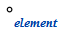
\includegraphics{images/5/scs/sentence}
  \caption{SCg-аналог для более сложного sc.s-предложения}
  \label{fig:SCs_sentence}
\end{figure}

Как можно заметить, <<\texttt{->}>> используется для обозначения
константной позитивной sc-дуги. Как видно из приведенного выше
рисунка, sc-элемент node является константным sc-узлом, а не
константным sc-элементом неопределенного вида. Это происходит потому,
что из node есть выходящая sc-дуга, поэтому он является sc-узлом.

Аналогом рассматриваемого текста является:
\begin{verbatim}
element <- node;
\end{verbatim}

Все то же самое, просто поменяли местами элементы и изменили
направление стрелки. В таблице 3.1 представлен полный перечень форм
записи различных видов sc-дуг на SCs.

Таблица 3.1 Соответствие SCg-изображения sc-дуги записи на SCs
Изображение на SCg  Запись на SCs (направления слева направо и справа налево)


Предложения на SCs могут иметь еще более сложную структуру, чем было
показано выше. Например:
\begin{verbatim}
node1, node2 -> element1, attr1_: attr2_: element2;
\end{verbatim}

Этот sc.s-текст соответствует sc.g-тексту, показанному на
рисунке~\ref{fig:SCs_sentence_with_attrs}. Как видите, sc-дуги
проводятся от \idtf{node1} и \idtf{node2} и к \idtf{element1}, и к
\idtf{element2}. А к sc-дугам, которые входят в \idtf{element2},
добавляются атрибуты \idtf{attr1\_} и \idtf{attr2\_} (для этого
используется символ <<\texttt{:}>>).

\begin{figure}[h!]
  \centering
  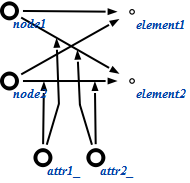
\includegraphics{images/5/scs/sentence_with_attrs}
  \caption{SCg-аналог для сложного sc.s-предложения c атрибутами}
  \label{fig:SCs_sentence_with_attrs}
\end{figure}

Для того чтобы задавать более удобно множества, можно использовать
следующую запись:
\begin{verbatim}
{a, attr1_: b, attr1_: attr3_: c};
\end{verbatim}

Этот sc.s-текст соответствует sc.g-тексту, показанному на
рисунке~\ref{fig:SCs_set}. Как видно из рисунка.

\begin{figure}[h!]
  \centering
  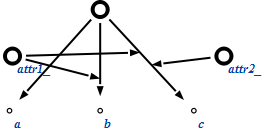
\includegraphics{images/5/scs/set}
  \caption{SCg-аналог для задания множества без идентификатора}
  \label{fig:SCs_set}
\end{figure}

%%% Local Variables: 
%%% mode: latex
%%% TeX-master: "ai_rr"
%%% End: 
